% xelatex
\documentclass[11pt,a4paper]{article}
\usepackage{geometry}
\usepackage{graphicx}
\usepackage{float}
\usepackage{amsmath,amssymb,amsfonts,amsthm}
\usepackage{mathtools}
\usepackage[dvipsnames,svgnames]{xcolor}
\usepackage{enumerate}
\usepackage[inline]{enumitem}
\usepackage{fancyhdr}
\usepackage{ragged2e}
\usepackage{titling}
\usepackage{hyperref}
\usepackage[numbers]{natbib}


% ---------- Preamble ----------
\pagestyle{fancyplain} % Make all pages in the document conform to the custom headers and footers
\fancyhead{} % No page header
\fancyfoot[L]{}
\fancyfoot[C]{}
\fancyfoot[R]{\thepage}
\renewcommand{\headrulewidth}{0pt} % Remove header underlines
\renewcommand{\footrulewidth}{0pt} % Remove footer underlines
\geometry{
    textwidth=160mm,
    top=25mm,
    bottom=25mm,
}
\setlist[enumerate]{
    label=\textnormal{(\arabic*)},
    topsep=0.5em,
    itemsep=0em,
}
\setlist[itemize]{
    topsep=0.5em,
    itemsep=0em,
}


% ---------- Theorem environments ----------
\theoremstyle{plain} % default
\newtheorem{theorem}{Theorem}
\newtheorem{corollary}[theorem]{Corollary}
\newtheorem{proposition}[theorem]{Proposition}
\newtheorem{lemma}[theorem]{Lemma}

\theoremstyle{definition}
\newtheorem{definition}[theorem]{Definition}

\theoremstyle{remark}
\newtheorem*{remark}{Remark}


% ---------- Symbol Macros ----------
\newcommand{\bra}[1]{\mathopen{}\left(#1\right)}
\newcommand{\sbra}[1]{\mathopen{}\left[#1\right]}
\newcommand{\cbra}[1]{\mathopen{}\left\{#1\right\}}
\newcommand{\abra}[1]{\mathopen{}\left\langle#1\right\rangle}
\newcommand{\norm}[1]{\mathopen{}\left\lVert#1\right\rVert}
\newcommand{\inp}[2]{\mathopen{}\left\langle#1,#2\right\rangle}
\newcommand{\abs}[1]{\mathopen{}\left|#1\right|}
\newcommand{\rest}[2]{\mathopen{}\left.#1\right|_{#2}}

\newcommand{\R}{\mathbb{R}}
\newcommand{\N}{\mathbb{N}}
\newcommand{\Z}{\mathbb{Z}}
\newcommand{\C}{\mathbb{C}}
\newcommand{\Q}{\mathbb{Q}}

\renewcommand{\d}{\mathrm{d}}
\newcommand{\dx}{\mathrm{d}x}
\newcommand{\dt}{\mathrm{d}t}
\newcommand{\dw}{\mathrm{d}W_t}
\newcommand{\E}{\mathbb{E}}
\renewcommand{\P}{\mathcal{P}}
\renewcommand{\N}{\mathcal{N}}
\renewcommand{\L}{\mathcal{L}}

\newcommand{\T}{\mathrm{T}}
\DeclareMathOperator{\spn}{span}
\DeclareMathOperator{\im}{im}
\DeclareMathOperator{\tr}{tr}
\DeclareMathOperator{\rank}{rank}

\def\ito{It\^{o}}
\newcommand{\KL}[2]{D_{\mathrm{KL}}\mathopen{}\left(#1\middle\|#2\right)}
\newcommand{\eps}{\epsilon_\theta(x_t,t)}
\newcommand{\sco}{s_\theta(x_t,t)}
\newcommand{\pmean}{\mu_\theta(x_t,t)}


% ---------- Title Section ----------
\title{Two Unified Perspectives on DDPM}
\author{Zhijie Chen}


\begin{document}
\maketitle

In this article, we introduce two different perspectives on Denoising Diffusion Probabilistic Models (DDPM): one from stochastic analysis (continuous-time Markov chains, CTMC), and one from discrete-time Markov chains (used by the original DDPM paper~\citep{ho2020denoising}). The material for the former is drawn from \citet{zhang2025aa7}.

\begin{figure}[H]
    \centering
    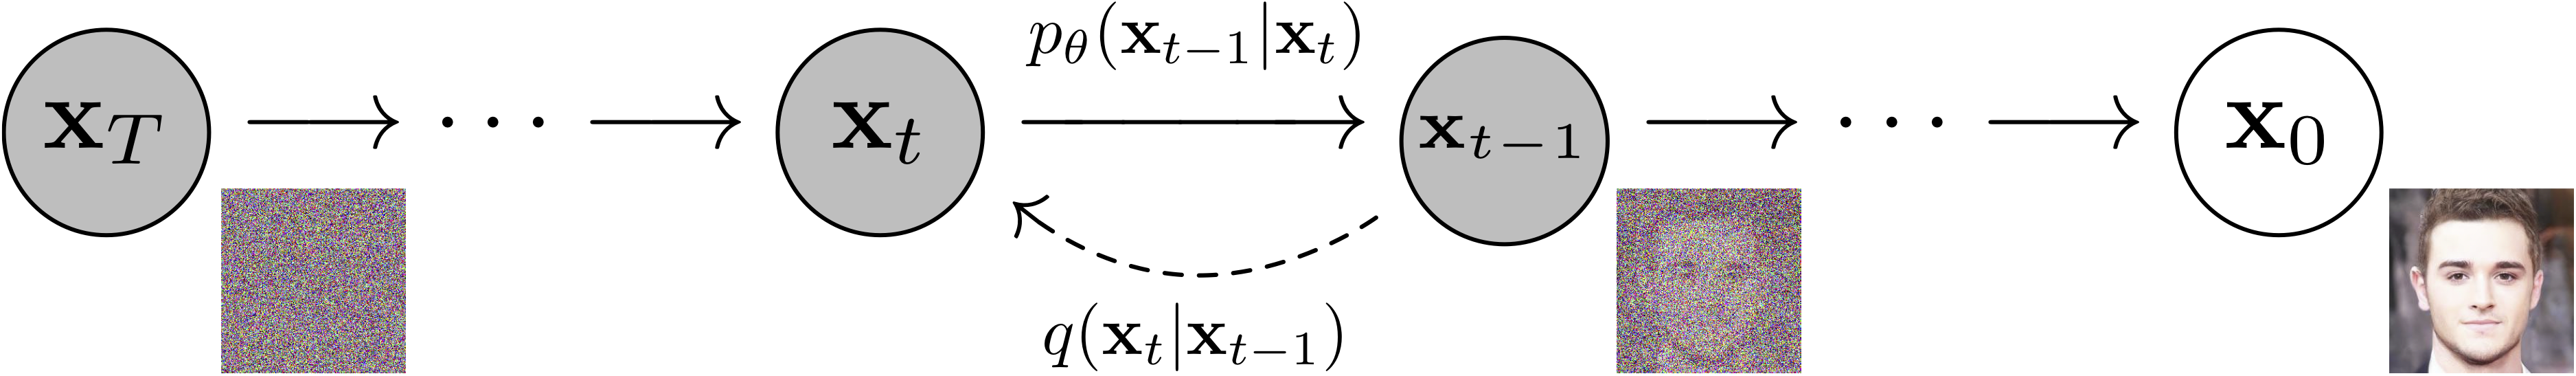
\includegraphics[width=0.7\textwidth]{ddpm.png}
    \caption{Forward diffusion and reverse denoising processes in DDPM~\citep{ho2020denoising}.}
\end{figure}

DDPM consists of two stages. The forward process systematically destroys a complex data sample by gradually adding Gaussian noise to it. The reverse process learns to denoise a noisy sample step by step to recover a sample from the data distribution (e.g., the uniform distribution on a large image dataset).

\section{The Stochastic Analysis Perspective}

\subsection{The forward process}

Consider an Ornstein--Uhlenbeck (OU) process
\begin{equation}\label{eq:ou}
    \d X_t = -X_t\,\dt + \sqrt2\,\dw,
\end{equation}
where $(W_t)_{t\ge0}$ is a standard Wiener process. Its solution is (by applying \ito's formula to $f(t,X_t)=e^tX_t$)
\begin{equation}\label{eq:ou_sol}
    X_t\overset{d}{=}e^{-t}X_0+\sqrt{1-e^{-2t}}\epsilon,\quad\epsilon\sim\N(0,I).
\end{equation}
As $t\to\infty$, $X_t$ converges in distribution to the standard Gaussian distribution. Hence, we can use \eqref{eq:ou_sol} to simulate the OU process and systematically destroy a data sample $X_0$.

\subsection{The reverse process}\label{sec:sa_reverse}

To learn the denoising process, consider the time-reversed process of \eqref{eq:ou}
\[Y_t=X_{T-t},\quad 0\le t\le T,\]
where $T$ is chosen sufficiently large such that the law of $X_T$ is close to the standard Gaussian distribution. A tedious calculation (see \citet{zhang2025sp14}) yields the SDE for the reverse process:
\begin{equation}\label{eq:reverse_ou}
    \d Y_t = (Y_t + 2\nabla\log\pi_{T-t}(Y_t))\,\dt + \sqrt2\,\d\bar W_t,
\end{equation}
where $\pi_t$ is the density of $X_t$.

To simulate \eqref{eq:reverse_ou} (e.g., using Euler--Maruyama discretization), it suffices to know the value of $\nabla\log\pi_t(x)$ (known as the score function) for every $t$ and $x$. However, this function is generally intractable to compute directly. So we approximate it using a neural network. The following formula makes it convenient to learn the score function.

\begin{theorem}[Tweedie's formula]\label{thm:tweedie}
    Let $Y = X + \sqrt t\cdot\epsilon$, where $\epsilon\sim\N(0,I)$ is independent of $X$. Let $p_Y$ be the density of $Y$. Then
    \[\E[X \mid Y=y] = y + t\nabla\log p_Y(y).\]
\end{theorem}

Recall from \eqref{eq:ou_sol} that
\[\underbrace{X_t}_Y = \underbrace{e^{-t}X_0}_X + \underbrace{\sqrt{1-e^{-2t}}}_{\sqrt t}\epsilon,\quad\epsilon\sim\N(0,I).\]
Since we can draw samples from the data distribution, we can construct $(x_0,x_t)$ pairs from the forward process, and train the network to predict $x_0$ from $x_t$ (and $t$). Use the ordinary MSE loss $\norm{x_0-\hat x_0}^2$. The solution to this easy optimization problem is
\[\hat x_0^*(x_t,t) = \E[x_0 \mid x_t].\]
Substituting it into Theorem~\ref{thm:tweedie} yields the score function.

\section{The Discrete-Time Markov Chain Perspective}

The original implementation of DDPM differs from the approach described above in several ways. In particular, it uses discrete-time Markov chains instead of \ito\ diffusions to model the forward and reverse processes.

\subsection{Noise schedule}

Instead of using a CTMC (OU process), the original DDPM selects a set of timesteps $(\tau_t)_{0\le t\le T}$ and only considers the discrete-time Markov chain $x_t = X_{\tau_t}$, $0\le t\le T$. Specifically, DDPM defines
\[0<\alpha_t<1,\quad \beta_t = 1-\alpha_t,\quad \bar\alpha_t=\prod_{s=1}^{t}\alpha_s,\quad 1\le t\le T,\]
\begin{equation}\label{eq:forward_one_step}
    x_t = \sqrt{\alpha_t}x_{t-1} + \sqrt{\beta_t}\epsilon,\quad\epsilon\sim\N(0,I).
\end{equation}
Or, equivalently,
\begin{equation}\label{eq:forward}
    x_t = \sqrt{\bar\alpha_t}x_0 + \sqrt{1-\bar\alpha_t}\epsilon,\quad\epsilon\sim\N(0,I).
\end{equation}
Set $\tau_t = -\frac12\log\bar\alpha_t$ and we can see that \eqref{eq:forward} is completely equivalent to \eqref{eq:ou_sol}. Hence, the noise schedule is just about selecting a discrete set of timesteps.

The original DDPM paper sets $T=1000$ and linearly increases $\beta_t$ from $10^{-4}$ to $0.02$. The smallness of $\beta_t$ will be used in the asymptotic expansion below.

\subsection{Prediction target}

DDPM usually directly predicts the noise in \eqref{eq:forward} using a neural network $\eps$. The ordinary MSE loss is used:
\[L_{\mathrm{simple}}=\E_{x_0,t,\epsilon}[\norm{\epsilon-\eps}^2],\quad t\sim\mathrm{Uniform}\{1,\dots,T\}.\]

We show that this new prediction target is essentially just a reparameterization of score matching. Let $\sco$ be the score estimator. The optimal noise predictor is $\epsilon^*(x_t,t)=\E[\epsilon\mid x_t]$. Take the conditional expectation of both sides of \eqref{eq:forward} given $x_t$, and combine it with Theorem~\ref{thm:tweedie}.
\begin{equation}\label{eq:score_x0_pred}
    \sco = -\frac\eps{\sqrt{1-\bar\alpha_t}},\qquad\hat x_0\coloneq\E[x_0\mid x_t]=\frac{x_t-\sqrt{1-\bar\alpha_t}\eps}{\sqrt{\bar\alpha_t}}.
\end{equation}
% \[\sco = -\frac\eps{\sqrt{1-\bar\alpha_t}},\]
% \begin{equation}\label{eq:x0_pred}
%     \hat x_0\coloneq\E[x_0\mid x_t]=\frac{x_t-\sqrt{1-\bar\alpha_t}\eps}{\sqrt{\bar\alpha_t}}.
% \end{equation}

\subsection{Gaussian posterior}

We will need the Gaussian posterior $q(x_{t-1}\mid x_t,x_0)$ in what follows.

\begin{align*}
    q(x_{t-1}\mid x_t,x_0) &= \frac{q(x_{t-1}\mid x_0)q(x_t\mid x_{t-1},x_0)}{q(x_t\mid x_0)} \\
    \text{\footnotesize(Markov property)}\quad &= \frac{q(x_{t-1}\mid x_0)q(x_t\mid x_{t-1})}{q(x_t\mid x_0)} \\
    &= \phi\bra{\frac{x_{t-1}-\sqrt{\bar\alpha_{t-1}}x_0}{\sqrt{1-\bar\alpha_{t-1}}}} \phi\bra{\frac{x_t-\sqrt{\alpha_t}x_{t-1}}{\sqrt{1-\alpha_t}}} \phi\bra{\frac{x_t-\sqrt{\bar\alpha_t}x_0}{\sqrt{1-\bar\alpha_t}}}^{-1} \\
    \text{\footnotesize(by a tedious calculation)}\quad &= \N(\tilde\mu_t,\tilde\beta_tI),
\end{align*}
where $\phi$ is the standard Gaussian density, and
\begin{equation}\label{eq:posterior}
    \tilde\mu_t=\frac{\sqrt{\bar\alpha_{t-1}}\beta_t}{1-\bar\alpha_t}x_0+\frac{\sqrt{\alpha_t}(1-\bar\alpha_{t-1})}{1-\bar\alpha_t}x_t,\qquad\tilde\beta_t=\frac{1-\bar\alpha_{t-1}}{1-\bar\alpha_t}\beta_t.
\end{equation}

\subsection{Sampling}

\subsubsection{Definition}

DDPM defines\footnote{Note that although $q(x_{t-1}\mid x_t,x_0)$ is Gaussian, $q(x_{t-1}\mid x_t)$ in general is not.}
\[p_\theta(x_{t-1}\mid x_t) = \N(\pmean,\sigma_t^2I),\]
where $\sigma_t^2$ usually equals $\beta_t$ or $\tilde\beta_t$, and
\begin{equation}\label{eq:post_mean}
    \pmean=\frac1{\sqrt{\alpha_t}}\bra{x_t-\frac{\beta_t}{\sqrt{1-\bar\alpha_t}}\eps}.
\end{equation}
Here $\pmean$ is obtained by substituting $\hat x_0$ for $x_0$ in \eqref{eq:posterior} (note that we no longer condition on $x_0$). During sampling, we start with $x_T\sim\N(0,I)$ and sample
\begin{equation}\label{eq:sample}
    x_{t-1} = \pmean + \sigma_tz,\quad t=T,\dots,1,
\end{equation}
where we resample $z\sim\N(0,I)$ at each step, and set $z=0$ at the final step $t=1$.

Note that although we substitute $\hat x_0$ for $x_0$ to obtain $\pmean$, which seems inaccurate, it still holds that $\mu^*(x_t,t)=\E[x_{t-1}\mid x_t]$:
\[\E[x_{t-1}\mid x_t] = \E[\E[x_{t-1}\mid x_t,x_0]\mid x_t] = \E[\tilde\mu_t\mid x_t] = \frac{\sqrt{\bar\alpha_{t-1}}\beta_t}{1-\bar\alpha_t}\hat x_0+\frac{\sqrt{\alpha_t}(1-\bar\alpha_{t-1})}{1-\bar\alpha_t}x_t=\mu^*(x_t,t).\]

\subsubsection{Connection to the reverse SDE}

We now show that the two perspectives are almost equivalent. Suppose $\sigma_t^2=\beta_t$. Combining \eqref{eq:sample}, \eqref{eq:post_mean}, and \eqref{eq:score_x0_pred} yields
\begin{align*}
    x_{t-1} &= \frac{x_t+\beta_t\sco}{\sqrt{1-\beta_t}} + \sqrt{\beta_t}z \\
    \text{\footnotesize(Taylor expand in $\beta_t$)}\quad &= x_t + \frac{\beta_t}{2}x_t + \beta_t\sco + O(\beta_t^2) + \sqrt{\beta_t}z \\
    \text{\footnotesize($h\coloneq\beta_t/2$)}\quad &\approx x_t + (x_t + 2\sco)h + \sqrt{2h}z.
\end{align*}
This coincides with the Euler--Maruyama discretization of \eqref{eq:reverse_ou}. Moreover, the step size $h$ also matches that in the discretized forward process \eqref{eq:forward_one_step}:
\[h_{\mathrm{forward}} = \tau_t - \tau_{t-1} = -\frac12\log(1-\beta_t)\approx\frac{\beta_t}{2}.\]

\subsection{Loss function}

\subsubsection{Reparameterization changes the loss weights across timesteps}

Section~\ref{sec:sa_reverse} uses equally weighted original-image MSE, while now we use equally weighted noise MSE. \eqref{eq:score_x0_pred} shows the difference between the two:
\[\norm{\epsilon-\epsilon_\theta}^2 = \frac{\bar\alpha_t}{1-\bar\alpha_t}\norm{x_0-\hat x_0}^2.\]
Therefore, noise MSE is the signal-to-noise ratio-weighted original-image MSE. The reparameterization changes the loss weights across timesteps and shifts the focus of training.

\subsubsection{An ELBO-based loss function}

We can use the evidence lower bound (ELBO) to derive an alternative loss function. To do this, define the model's joint distribution $p_\theta(x_{0:T})$ and the forward distribution $q(x_{1:T}\mid x_0)$. They factorize as
\begin{equation}\label{eq:factorize}
    p_\theta(x_{0:T}) = \phi(x_T)\prod_{t=1}^{T}p_\theta(x_{t-1}\mid x_t),\qquad q(x_{1:T}\mid x_0) = q(x_T\mid x_0)\prod_{t=2}^{T}q(x_{t-1}\mid x_t,x_0).
\end{equation}
Here we use the Markov property. Now ELBO gives

\begin{align*}
    \log p_\theta(x_0) &\ge \E_{q(x_{1:T}\mid x_0)}\sbra{\log\frac{p_\theta(x_{0:T})}{q(x_{1:T}\mid x_0)}} \\
    &= \E_{q(x_{1:T}\mid x_0)}\sbra{\log\frac{\phi(x_T)}{q(x_T\mid x_0)}+\sum_{t=2}^{T}\log\frac{p_\theta(x_{t-1}\mid x_t)}{q(x_{t-1}\mid x_t,x_0)}+\log p_\theta(x_0\mid x_1)} \\
    &= -L_{\mathrm{VLB}},
\end{align*}
where VLB stands for variational lower bound and
\[L_{\mathrm{VLB}} = \E\sbra{\underbrace{\KL{q(x_T\mid x_0)}{\phi(x_T)}}_{L_T} + \sum_{t=2}^{T}\underbrace{\KL{q(x_{t-1}\mid x_t,x_0)}{p_\theta(x_{t-1}\mid x_t)}}_{L_{t-1}} - \underbrace{\log p_\theta(x_0\mid x_1)}_{\text{reconstruction loss}}}.\]

Let's look at $L_T$ first. Because
\[q(x_T\mid x_0)=\N(\sqrt{\bar\alpha_T}x_0,(1-\bar\alpha_T)I),\qquad p(x_T)=\N(0,I),\]
$L_T$ does not depend on $\theta$ and thus can be ignored during training.

Now consider $L_{t-1}$. We already know that
\[q(x_{t-1}\mid x_t,x_0)=\N(\tilde\mu_t,\tilde\beta_tI),\qquad p_\theta(x_{t-1}\mid x_t)=\N(\mu_\theta,\sigma_t^2I).\]
Hence
\[D_{\mathrm{KL}}=\frac{\norm{\tilde\mu_t-\mu_\theta}^2}{2\sigma_t^2}+\underbrace{\frac d2\bra{\frac{\tilde\beta_t}{\sigma_t^2}-1+\log\frac{\sigma_t^2}{\tilde\beta_t}}}_{\text{not depending on $\theta$}}.\]
\[L_{t-1}=\E_{x_0,\epsilon}\sbra{\frac{\beta_t^2}{2\sigma_t^2\alpha_t(1-\bar\alpha_t)}\norm{\epsilon-\eps}^2}+C_t.\]
Here $d$ is the data dimension and $C_t$ is a constant that does not depend on $\theta$.

Now consider the reconstruction loss. Direct calculation yields
\[L_0=\E_{x_0,\epsilon}\sbra{\frac{\beta_1}{2\sigma_1^2\alpha_1}\norm{\epsilon-\eps}^2}+C.\]

Note that in the original DDPM implementation, $L_{\mathrm{simple}}$ is adopted instead of this fancier ELBO-based loss $L_{\mathrm{VLB}}$, because the former just works better.

\bibliographystyle{plainnat}
\bibliography{references}

\end{document}